% DO NOT COMPILE THIS FILE DIRECTLY!
% This is included by the other .tex files.

\begin{frame}[t,plain]
\titlepage
\end{frame}

\section{Introduction}
\begin{frame}
        \frametitle{Concepts - Deep Web}
        \begin{itemize}
                \item {\bf Deep Web} is the part of World Wide Web not indexed or directly accessible by standard web search-engines;
                \item This can be content hidden from {\bf crawlers} by requiring a specific access and this can includes private social media, password-protected forums or content protected
                        by different measures such as paywalls or specific security interface to access the information;
                \item A large portion of content accessible via Internet is part of the deep web\footnote{also called invisible web, hidden web or non-indexed web}.
        \end{itemize}
        \note[item]{There is a huge misconception about the difference between the darknet and deep web. The differences are important because it's two different aspects which can be related to each other.}
\end{frame}

\begin{frame}
        \frametitle{Concepts - darknet}
        \begin{itemize}
                \item {\bf Darknet} is an overlay network running on top of Internet requiring specific software to access the network and its services;
                \item Tor, I2P and Freenet are the most commonly used ones. Many are used for hidden services access and some for proxy access to the Internet;
		\item There are {\bf legitimate use-cases} for such network but also many {\bf illegal or criminal usage}.
        \end{itemize}
\end{frame}

\begin{frame}
	\frametitle{Lifecycle of collection and analysis}
	\center
\tikzstyle{startstop} = [rectangle, rounded corners, minimum width=3cm, minimum height=0.8cm,text centered, draw=black, fill=white!10]
\tikzstyle{io} = [trapezium, trapezium left angle=70, trapezium right angle=110, minimum width=3cm, minimum height=1cm, text centered, draw=black, fill=blue!30]
\tikzstyle{arrow} = [thick,->,>=stealth]
	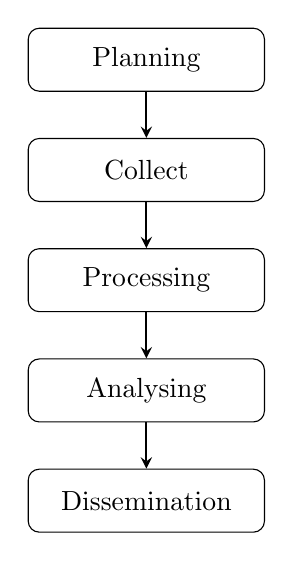
\begin{tikzpicture}[node distance=1.4cm]

\node (start) [startstop] {Planning};
\node (collect) [startstop, below of =start] {Collect};
\node (processing) [startstop, below of =collect] {Processing};
\node (analysing) [startstop, below of=processing] {Analysing};
\node (dissemination) [startstop, below of=analysing] {Dissemination};
\draw [arrow] (start) -- (collect);
\draw [arrow] (collect) -- (processing);
\draw [arrow] (processing) -- (analysing);
\draw [arrow] (analysing) -- (dissemination);
%\draw [arrow] (analysing) |- (collect);
\end{tikzpicture}

\end{frame}

\begin{frame}
        \frametitle{Collecting, processing and analysing content - web pages}
        \begin{itemize}
		\item Building a search engine on the web is a challenging task because:
        	\begin{itemize}
			\item it has to crawl webpages,
			\item it has to to make sense of {\bf unstructured data},
			\item it has to {\bf index} these data,
			\item it has to provide a way to retrieve data and structure data (e.g. correlation).
        	\end{itemize}
		\item Doing so on Tor is even more challenging because:

        	\begin{itemize}
			\item services don't always want to be found,
			\item parts of the dataset have to be discarded.
        	\end{itemize}
	\item in each case, it requires a lot of bandwidth, storage and computing power.
        \end{itemize}
\end{frame}

\begin{frame}
        \frametitle{Collecting, processing and analysing content - structured data}
        \begin{itemize}
		\item Some data are structured and are easy to process:
        	\begin{itemize}
			\item metadata!
			\item API responses.
        	\end{itemize}
		\item Some even provide cryptographic evidences:
			        \begin{itemize}

         \item authentication mechanisms between peers,
         \item OpenGPG can leak a lot of metadata
        \begin{itemize}
          \item key ids,
          \item subject of email in thunderbird,
        \end{itemize}
          \item Bitcoin's Blockchain is public,
          \item pivoting on these data with external sources yields interesting results.
        \end{itemize}
        \end{itemize}
\end{frame}

\section{AIL design Objectives}
\begin{frame}
\frametitle{Objectives of the session}
    \begin{itemize}
        \item Show how to use and extend an open source tool to monitor web pages, pastes, forums and hidden services
        \item Explain challenges and the design of the AIL open source framework
        \item Review different {\bf collection mechanisms} and {\bf sources}
        \item Learn how to create new modules
        \item Learn how to use, install and start AIL
        \item {\bf Supporting investigation using the AIL framework} and including it in cyber threat intelligence lifecycle
    \end{itemize}
\end{frame}

\section{AIL Framework}
\begin{frame}
    \frametitle{From a requirement to a solution: AIL Framework}
    \large{History:}
    \begin{itemize}
        \item AIL initially started as an \textbf{internship project} (2014) to evaluate the feasibility to automate the analysis of (un)structured information to find leaks.
        \item In 2019, AIL framework is an \textbf{open source software} in Python. The software is actively used (and maintained) by CIRCL and many organisations.
        \item In 2020, AIL framework is now a complete project called \textbf{ail project}\footnote{\url{https://github.com/ail-project/}}.
    \end{itemize}
\end{frame}

\section{Capabilities Overview}

\begin{frame}
    \frametitle{Common usage}
        \begin{itemize}
                \item {\bf Check} if mail/password/other sensitive information (terms tracked) leaked
                \item {\bf Detect} reconnaissance of your infrastructure
                \item {\bf Search} for leaks inside an archive
                \item {\bf Monitor} and crawl websites
        \end{itemize}
\end{frame}

\begin{frame}
    \frametitle{Support CERT/CSIRTs and Law Enforcement activities}
        \begin{itemize}
            \item Proactive investigation: leaks detection
            \begin{itemize}
		        \item List of emails and passwords
		        \item Leaked database
		        \item AWS Keys
		        \item Credit-cards
		        \item PGP private keys
		        \item Certificate private keys
		    \end{itemize}
		    \item Feed Passive DNS or any passive collection system
		    \item CVE and PoC of vulnerabilities most used by attackers
		\end{itemize}
\end{frame}

\begin{frame}
    \frametitle{Support CERT/CSIRTs and Law Enforcement activities}
    	\begin{itemize}
		    \item Website monitoring
		    	\begin{itemize}
				    \item monitor booters
                    \item Detect encoded exploits (WebShell, malware encoded in Base64...)
				    \item SQL injections
		    	\end{itemize}
		    \item Automatic and manual submission to threat sharing and incident
response platforms
			\begin{itemize}
				\item MISP
				\item TheHive
			\end{itemize}
		    \item Term/Regex/Yara monitoring for local companies/government
        \end{itemize}
\end{frame}

\begin{frame}
    \frametitle{Sources of leaks: Paste monitoring}
    \begin{itemize}
        \item Example: \url{https://gist.github.com/}
            \begin{itemize}
                \item Easily storing and sharing text online
                \item Used by programmers and legitimate users
                \item[] $\to$ Source code \& information about configurations
            \end{itemize}
        \pause
        \item Abused by attackers to store:
            \begin{itemize}
                \item List of vulnerable/compromised sites
                \item Software vulnerabilities (e.g. exploits)
                \item Database dumps
                \item[] $\to$ User data
                \item[] $\to$ Credentials
                \item[] $\to$ Credit card details
                \item More and more ...
            \end{itemize}
    \end{itemize}
\end{frame}

\begin{frame}
        \frametitle{Why so many leaks?}
        \begin{itemize}
                \item Economical interests (e.g. Adversaries promoting services)
                \item Ransom model (e.g. To publicly pressure the victims)
                \item Political motives (e.g. Adversaries showing off)
                \item Collaboration (e.g. Criminals need to collaborate)
                \item Operational infrastructure (e.g. malware exfiltrating information on a pastie website)
                \item Mistakes and errors
        \end{itemize}
\end{frame}


\begin{frame}
    \frametitle{Are leaks frequent?}
    \begin{center}
    \Large{Yes!}\\ and we have to deal with this as a CSIRT.
    \end{center}

    \begin{itemize}
            \item {\bf Contacting companies or organisations} who did specific accidental leaks
            \item {\bf Discussing with media} about specific case of leaks and how to make it more practical/factual for everyone
            \item Evaluating the economical market for cyber criminals (e.g. DDoS booters\footnote{\url{https://github.com/D4-project/}} or reselling personal information - reality versus media coverage)
            \item Analysing collateral effects of malware, software vulnerabilities or exfiltration
    \end{itemize}

    \begin{center}
    $\rightarrow$ And it's important to detect them automatically.
    \end{center}
\end{frame}

\begin{frame}
    \frametitle{Paste monitoring at CIRCL: Statistics}
    \begin{itemize}
        \item Monitored paste sites: 27
            \begin{itemize}
                \item \textit{gist.github.com}
                \item \textit{ideone.com}
                \item \textit{...}
            \end{itemize}
    \end{itemize}
    \begin{table}[h]
		\centering
		\begin{tabular}{|lrrr|}
		    \hline
		    \rowcolor{lightgray} & 2016 & 2017 & 08.2018\\
		    Collected pastes & 18,565,124 & 19,145,300 & 11,591,987 \\
		    Incidents & 244 & 266 & 208\\
		    \hline
		\end{tabular}
		\caption{Pastes collected and incident\footnote{\url{http://www.circl.lu/pub/tr-46}} raised by CIRCL}
		\label{circlStats}
	\end{table}
\end{frame}



